\documentclass{standalone}
\usepackage{tikz}
\usetikzlibrary{shapes.geometric, arrows}

\definecolor{pantone}{RGB}{63,173,168}
\definecolor{red}{RGB}{255,0,0}
\tikzstyle{blockblack} = [rectangle, rounded corners, minimum width=6cm, minimum height=1.5cm,text centered, draw=black, fill=pantone]
\tikzstyle{blockred} = [rectangle, rounded corners, minimum width=6cm, minimum height=1.5cm,text centered, draw=red, fill=pantone, ultra thick]
\tikzstyle{arrow} = [thick,->,>=stealth]

\begin{document}

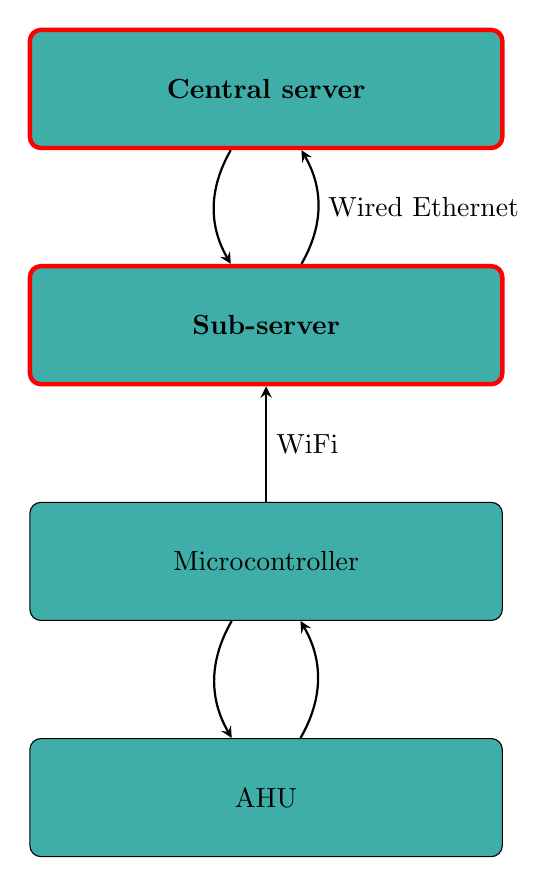
\begin{tikzpicture}[node distance=3cm]

\node (centralserver) [blockred] {\textbf{{Central server}}};
\node (subserver) [blockred, below of=centralserver] {\textbf{{Sub-server}}};
\node (microcontroller) [blockblack, below of=subserver] {Microcontroller};
\node (ahu) [blockblack, below of=microcontroller] {AHU};

\draw [arrow, bend right] (centralserver) edge (subserver);
\draw [arrow, bend right] (subserver) edge node[anchor=west] {Wired Ethernet} (centralserver);
\draw [arrow] (microcontroller) edge node[anchor=west] {WiFi} (subserver);
\draw [arrow, bend right] (microcontroller) edge (ahu);
\draw [arrow, bend right] (ahu) edge (microcontroller);

\end{tikzpicture}

\end{document}